%!TEX root = ../iceDetection.tex

\documentclass[a4paper,14pt]{extarticle}

\usepackage{cmap}
\usepackage[T2A]{fontenc}
\usepackage[utf8x]{inputenc}
% \usepackage{mathptmx}
\usepackage[english, russian]{babel}

\usepackage{misccorr}
\usepackage{amssymb,amsfonts,amsmath,amsthm}  
\usepackage{indentfirst}
\usepackage[usenames,dvipsnames]{color} 
\usepackage[unicode,hidelinks]{hyperref}
\usepackage{makecell,multirow} 
\usepackage{ulem}
\usepackage{graphicx,wrapfig}
\graphicspath{{img/}}

\renewcommand{\labelenumii}{\theenumii)} 
\newcommand{\mean}[1]{\langle#1\rangle}

\DeclareMathOperator{\Div}{div}
\DeclareMathOperator{\const}{const}
%%%%%%%%%%%%%%%%%%%%%%%%%%%%%%%%%%%%%%%%%%%%%%%%%%%%%%%%%%%%%%%%%%%%%%%%%%%%%%%
%%%%%%%%%%%%%%%%%%%%%%%%%%%%%%%%%%%%%%%%%%%%%%%%%%%%%%%%%%%%%%%%%%%%%%%%%%%%%%%
\usepackage{float}
\usepackage[mode=buildnew]{standalone}
\usepackage[outline]{contour}
\usepackage{tocloft}
\renewcommand{\cftsecleader}{\cftdotfill{\cftdotsep}} % for parts
% \renewcommand{\cftchapleader}{\cftdotfill{\cftdotsep}} % for chapters
\usepackage{pgfplots,pgfplotstable,booktabs,colortbl}
\usepackage{physics}
\usepackage{mathtools}
% \mathtoolsset{showonlyrefs=true}

% \newcommand*\dotvec[1][1,1]{\crossproducttemp#1\relax}
% \def\crossproducttemp#1,#2\relax{{\qty[\vec{#1}\times\vec{#2}\,]}}

% \newcommand*\prodvec[1][1,1]{\crossproducttempa#1\relax}
% \def\crossproducttempa#1,#2\relax{{\qty[{#1}\times{#2}\,]}}
% \usepackage{showframe}
\usepackage[]{geometry}
\geometry{
  left=2.5cm,
  right=1.5cm,
  top=2cm,
  bottom=2cm,
  bindingoffset=0cm,
  headheight=17pt
}
\linespread{1.5} 
\setlength{\parindent}{1.25cm}
\frenchspacing 
\usepackage{setspace}
\setlength{\tabcolsep}{20pt}
\renewcommand{\arraystretch}{1.5}
\usepackage{xcolor}



\begin{document}

%!TEX root = ../iceDetection.tex
\begin{titlepage}
	\begin{center}
	  {\fontsize{ 12pt }{ 12pt } \selectfont \bf 
	  МИНИСТЕРСТВО НАУКИ И ВЫСШЕГО ОБРАЗОВАНИЯ \\[-10pt] 
	  РОССИЙСКОЙ ФЕДЕРАЦИИ}\\
	  \vspace{12pt}
	  \begin{spacing}{1}
		{\bf  Федеральное государственное автономное \\
		образовательное учреждение высшего образования \\
		<<Национальный исследовательский \\ 
		Нижегородский государственный университет им. Н.И. Лобачевского>>
		}
	  \end{spacing}
	  \vspace{24pt}
	  \begin{spacing}{1}
		Радиофизический факультет\\
		Кафедра общей физики\\
		\vspace{20pt}
		Направление <<Радиофизика>>\\
		\vspace{20pt}
		{ \fontsize{18pt}{18pt}ОТЧЕТ ПО УЧЕБНОЙ ПРАКТИКЕ}\\
		(Практика по получению первичных профессиональных умений и навыков, в том числе первичных умений и навыков научно-исследовательской деятельности\\
		% \vspace{20pt}
		% { \fontsize{18pt}{18pt} \bf Детектирование ледяного покрова по данным двухчастотного радиолокатора}
	  \end{spacing}
	  \vspace{100pt}
	  
		\begin{align*}
		  &\text{Руководитель практики:}\quad &\text{Панфилова М.\,А.}\\
		  &\text{Студент 3-го курса бакалавриата:}\quad &\text{Шиков А.\,П.}
		\end{align*}
	 
	\end{center}
	\vfill
	\begin{center}
	  {Нижний Новгород, 2019}
	\end{center}
  \end{titlepage}



\tableofcontents
\newpage
\section{Введение}
% \addcontentsline{toc}{section}{Введение}

Мониторинг ледяного покрова является важной задачей для решения как научных так и практических проблем. Он широко
применяется в мореходстве, предсказании изменений климата и погоды, а также для решения различных фундаментальных задач.
Спутниковое наблюдение обладает огромными возможностями в реализации мониторинга интересующих областей.
Это может быть оптическое наблюдение, например в ясную погоду лед хорошо виден с оптических снимков, однако во время
облачности этот способ по понятным причинам не подходит. Помимо оптики, используются пассивные методы радиометрии –
радиометры, и активные методы, такие как РСА и альтиметры. Однако исследованиями практически не охвачены, за исключением
альтиметра, диапазоны малых и средних углов падения от 0 $^{\circ}$ до 18$^{\circ}$.

\textbf{Цель работы} - исследование методов детектирования льда на поверхности моря по данным для малых и средних углов падения,
используя данные двухчастотного радиолокатора, установленного на спутнике GPM (Global Precipitation Measurment).


\section{Миссия GPM}
Спутник миссии Global Precipitation Measurment[ссылка?] был запущен в феврале 2014 для обнаружения атмосферных осадков.
Он оборудован микроволновым формирователем изображений (GMI, радиометр), а также двухчастотным радаром (Dual frequency
Precipitation Radar - DPR). 

Радар работает в Ku(13.6 ГГц) и Ka(35.5 ГГц) диапазоне частот. Сканирование производится перпендикулярно направлению
полета, с максимальным отклонением до 18° у Ku диапазона, и до ??° у Ka диапазона. В таблице ?? приведена некоторая
техническая информация о радаре.
Ширина полосы обзора составляет 245 км, со средним разрешением 5 км.

Ku и Ka диапазоны радара выравнены, и измеряемые области совпадают для двух частот.  

В ходе нескольких исследований [??вставить ссылка на работы В.Ю., Маши ], было показано, что двухчастотный радар
чувствителен не только к осадкам, но и к типу отражающей поверхности. В частности, в \cite{kar1} описывалось отличие
отраженного сигнала от поверхности воды и от поверхности льда.


\section{Теория}

\subsection{Краткая теория радара}
\begin{figure}[h!]
  \centering
  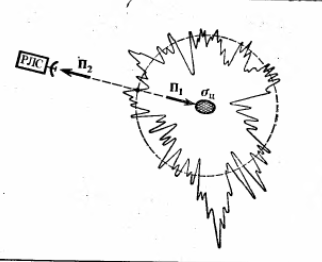
\includegraphics[width = .6\linewidth]{img/sigma0melnik.png}
  \caption{К формуле \eqref{eq:1.1}}
  \label{fig:1}
\end{figure}
Радар собирает информацию о величине сечения обратного рассеяния. 
Объект радиолокационного наблюдения можно охарактеризовать отношением напряженностей поля или плотностей потока мощности
отраженной волны и зондирующего колебания. В радиолокации характеристикой отражения сосредоточенной цели
является \textit{эффективная площадь}, или эффективная площадь рассеяния (ЭПР)\cite{meln}:
\begin{equation}
  \sigma = 4 \pi R^2 \frac{\Pi_2}{\Pi_1}
  \label{eq:1.1}
\end{equation}
Где $\Pi_1$ – плотность потока мощности падающей волны вблизи цели, а $\Pi_2$ – плотность потока мощности отраженной
волны, принятой РЛС, R - расстояние от РЛС до цели. (Множитель $4 \pi R^2$  исключает зависимость отношения плотностей потока от
расстояния.) ЭПР сильно зависит от формы, ориентации и материала облучаемого объекта. В нашем случае, когда тело имеет
большие размеры, имеет смысл ввода элементарной площадки S, и говорить не об эффективной площади, а об удельной
эффективной площади рассеяния, обозначаемой $\sigma^0$ (УЭПР) :
\begin{equation}
  \sigma^0 = 4 \pi R^2 \frac{\Pi_2}{S\Pi_1} = \gamma \cos \theta
  \label{eq:1.2}
\end{equation}
(Где угол $\theta$ – угол между направлением распространения и нормалью к площадке S.)

\subsection{Квазизеркальное приближение}
Если рассматривать с точки зрения теории, какую УЭПР должна иметь поверхность, например, воды, то наблюдаемое на
практике распределение достаточно хорошо описывается квазизеркальным приближением, в которой вводится двухмасштабная
модель поверхности - гладкая поверхность, покрытая рябью. Крупномасштабная поверхность разбивается на
фасеты, и при отражении, вклад вносят только площадки, расположенные перпендикулярно к вектору падающей волны, а рябь
влияет только на коэффициент отражнения от них.

\begin{figure}[h!]
  \centering
  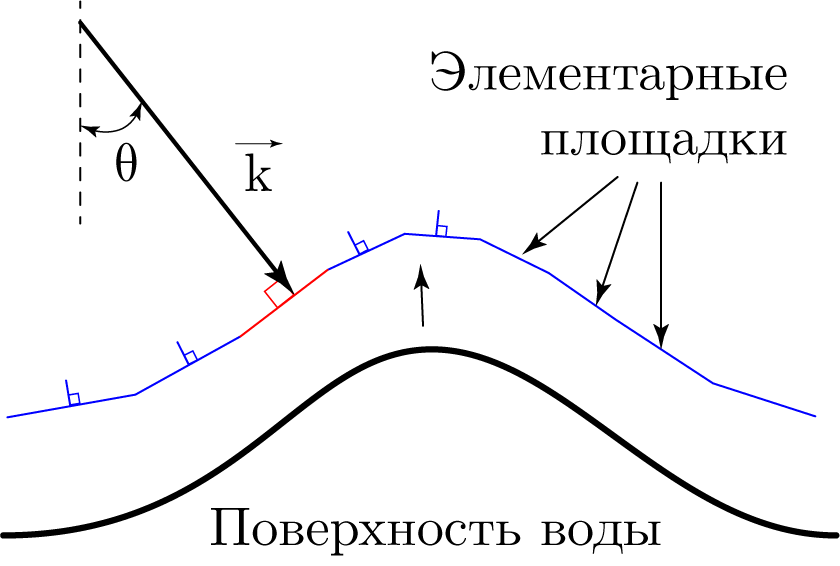
\includegraphics[width = .45\linewidth]{img/kvaz.png}
  \caption{}
  \label{fig:2}
\end{figure}

\textcolor{red}{!!! добавить из Машиного артикла}
Для воды зависимость сечения рассеяния от угла падения пропорциональна плотности распределения зеркальных площадок
$P(\tan \theta)$  \cite{bassfuks}:
\begin{equation}
  \sigma^0 = A (\cos \theta)^{-4} \cdot P(\tan \theta)
  \label{eq:3}
\end{equation}
, где $\theta$ - угол отклонения от нормали(А – эффективный коэффициент отражения, на величину которого влияет наличие
ряби). Для воды такая плотность имеет вид нормального распределения[??ссылку]:
\begin{equation}
  P_w(\tan \theta) = \frac{1}{\sigma_x \sqrt{2 \pi}} \cdot \exp (- \frac{\tan^2\theta}{2 \sigma^2_x})
  \label{eq:4}
\end{equation}
где $\sigma_x$ - дисперсия уклонов морской поверхности, зависящая, в частности, от скорости ветра.

\section{Анализ данных}
Для разработки метода детектирования льда, необходимо понять, чем ледяной покров отличается от водной поверхности на
изображении двухчастотного радиолокатора. На рис. \ref{fig:3} приведены изображения охотского моря за 27 декабря 2016
года в оптическом диапазоне, а также трек спутниковых данных Ku-диапазона радара DPR за тот же день.

\begin{figure}[h!]
  \centering
  \begin{minipage}{.49\linewidth}
    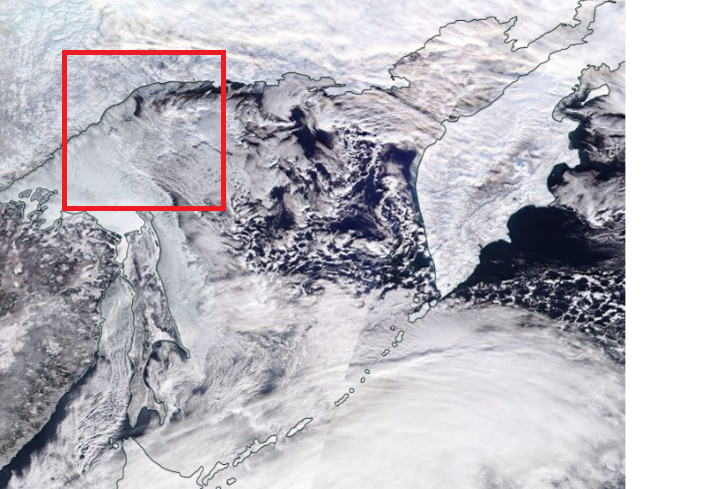
\includegraphics[width = \linewidth]{pic1.png}
  \end{minipage}
  \begin{minipage}{.49\linewidth}
    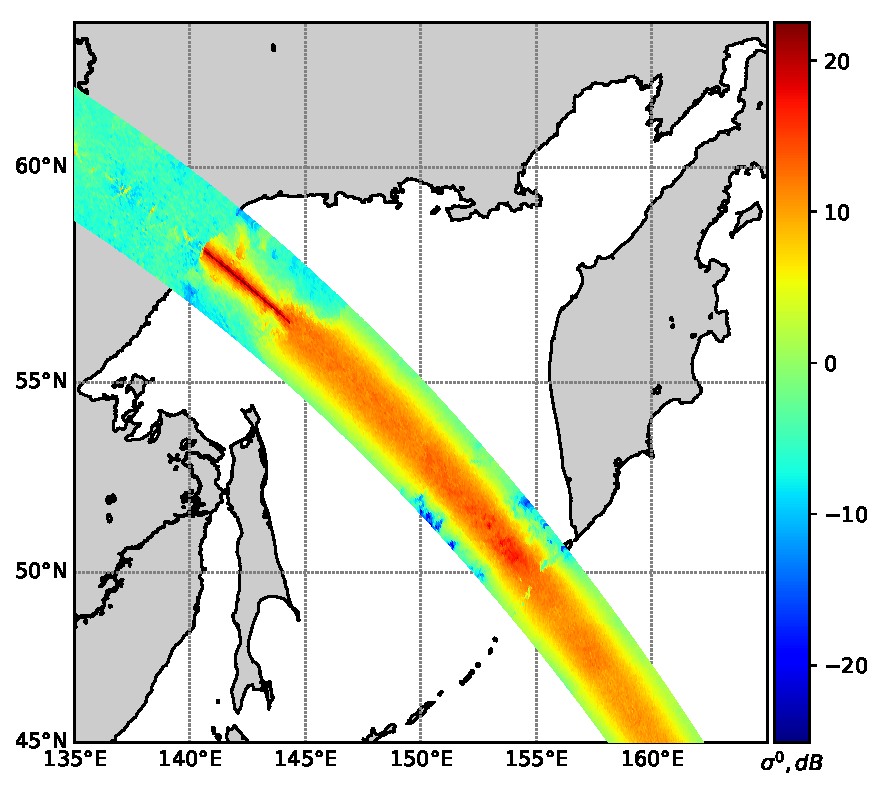
\includegraphics[width = \linewidth]{plot.pdf}
  \end{minipage}
  \caption{27.12.2016. Слева - спутниковое изображение, справа - трек Ku-диапазона DPR (цветом обозначена $\sigma^0$ в дБ).}
  \label{fig:3}
\end{figure}

В области, обведенной красной рамкой (на снимке), присутствует ледяной покров. Через эту область также проходит трек
спутниковых данных, и наблюдаются характерные отличия в данных для обасти, покрытой льдом. Если рассматривать поперечные
разрезы трека, т.е. угловую зависимость величины $\sigma^0(\theta)$, то мы получим картину на рис. \ref{fig:4}(слева), где
разные кривые соответствуют двум разным местам поперечного разреза, отмеченные на треке как две прямые линии
соответствующего цвета(черный - лед, красный - вода).

\begin{figure}[h!]
  \centering
  \begin{minipage}{.49\linewidth}
    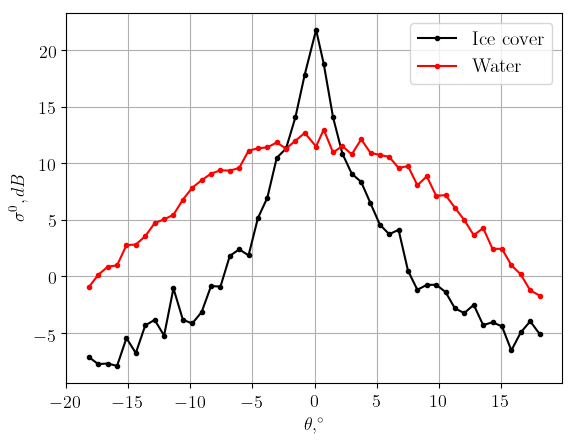
\includegraphics[width = \linewidth]{ice_cuts.png}
  \end{minipage}
  \begin{minipage}{.49\linewidth}
    \includegraphics[width = \linewidth]{plot_zoomed.pdf}
  \end{minipage}
  \caption{Слева - зависимости $\sigma^0(\theta)$ для поверхности льда(черный) и воды(красный), справа - трек Ku-диапазона, с отмеченными местами разрезов. }
  \label{fig:4}
\end{figure}

Как видно из рис. \ref{fig:4}, наблюдается существенная разница между зависимостями для поверхности льда и воды. Лед, по
отношению к воде, имеет б\'{о}льшие значения при малых углах падения и меньшие значения при больших, в то время как вода
имеет достаточно плавное распределение. Такую зависимость для льда можно объяснить достаточно просто в рамках
квазизеркального приближения. Так как лед - это достаточно гладкая поверхность, то при малых углах падения количество
перпендикулярных площадок намного больше, чем у воды, на которой постоянно присутствуют волнения. Следствием из этого
является большая отраженная энергия, а значит, и большее значение $\sigma^0$. 

При увеличении угла отклонения, количество зеркальных площадок на поверхности льда быстро спадает, и характер отражения сигнала
сменяется с квазизеркального на диффузный. При этом также быстро спадает количество отраженной энергии и велична УЭПР,
поэтому наблюдается такое резкое спаданение сигнала.

При анализе большого количества разрезов для ледяного покрова, все  угловые зависимости имели выделенный пик при нулевом
угле падения. Этот факт было решено использовать, как метод отличия ледяной поверхности от водной. В частности, для
того, чтобы определить, насколько выделенный пик имеет распределение, используется коэффициент эксцесса $\gamma_2$:
\begin{equation}
  \gamma_2 = \frac{\mu_4}{\sigma^4} -3
  \label{eq:5}
\end{equation}
,где $\mu_4$ - четвертый центральный момент, а $\sigma^2 = \mu_2$ - дисперсия. Для случайной величнины $x$ с известной плотностью вероятности $f(x)$, k-й
центральный момент это:
\begin{equation}
  \mu_k = \int \limits_{-\infty}^{\infty}(\overline{x}-x)^k f(x) dx
  \label{eq:6}
\end{equation} 
, где $\overline{x}$ - среднее значение величины $x$:
\begin{equation}
  \overline{x} = \int \limits_{-\infty}^{\infty}x f(x) dx
  \label{eq:7}
\end{equation}

 

\section{Разработка}
Разработка велась на языке программирования Python и его библиотеках. Как было описано ранее, в работе использовались
данные радиолокатора DPR, которые находятся в свободном доступе, и могут
быть предоставленны по запросу с \cite{data} в формате HDF5. Структура данных выглядит следующим образом:
\begin{figure}[h!]
  \centering
  \includegraphics[width = 0.55\linewidth]{example-image-a}
  \caption{Структура данных}
  \label{fig:5}
\end{figure}

В файле .HDF5 содержатся массивы данных для координат - долгот\'{ы} и широт\'{ы}, угла падения, и значение $\sigma^0_{dB}$ в
дБ. 

\subsection{Методы валидации}

Для валидации методов детектирования использовались размеченные карты НИЦ «Планета» в виде полигонов областей и информацию об их содержании
- тип, возраст, сплоченость льда и др.. Зная координаты точки, ее значение $\sigma^0$ и угла падения, а также полигона,
которому она принадлежит, существующие данные можно разметить для валидации после работы алгоритма. 

Также для валидации использовались данные с радиометра(GMI), расположенного на том же спутнике.  

Имея размеченные треки, мы можем сравнить их с данными радиометра, расположенного на том же спутнике, а также с
картами «Планета».


\subsection{Коэффициент эксцесса}

Коэфиициента эксцесса $\gamma_2$ рассчитывается для плотности распределения зеркальных площадок $P(\tan \theta)$. При этом: 
\begin{equation}
  \sigma^0 = A \cos^{-4}(\theta) \cdot P(\tan \theta)
  \label{eq:8}
\end{equation}
Учитывая, что данные имеют значение для $\sigma^0_{dB}$ в дБ, то чтобы получить значение $P(\tan \theta)$ необходимо сделать
соответствующие преобразования:
\begin{equation}
  P(\tan \theta) =  \frac{\sigma^0 \cos^4(\theta)}{A},~ \sigma^0 = 10^{\frac{\sigma^0_{dB}}{10}}
  \label{eq:9}
\end{equation}

Для рассчета $\gamma_2$ необходимо рассчитать 2-й и 4-й центральные моменты для величины $\tan \theta$ и плотности $P(\tan \theta)$:
\begin{equation}
  \mu_k = \int \limits_{-\infty}^{\infty}(\overline{\tan \theta}-\tan \theta)^k P(\tan \theta) d(\tan \theta)
  \label{eq:10}
\end{equation} 
или в дискретном случае для $N = 49$ точек:
\begin{equation}
  \mu_k = \sum \limits_{n = 1}^{N} (\overline{\tan\theta} - \tan \theta_n)^k ~P(\tan \theta_n) \Delta(\tan \theta_n)
  \label{eq:11}
\end{equation} 
\begin{equation}
  \mu_k = \sum \limits_{n = 1}^{N} (\overline{\tan\theta} - \tan \theta_n)^k~ \frac{\sigma^0_n \cos^4(\theta_n)}{A} \Delta(\tan \theta_n)
  \label{eq:12}
\end{equation}
Для рассчета коэффициента $A$ воспользуемся нормирокой плотности распределения $P(\tan \theta)$:
\begin{equation}
  \int \limits_{-\infty}^{\infty} f(x)dx = 1 \Rightarrow \int \limits_{-\infty}^{\infty} P(\tan \theta) d(\tan \theta) = 1
  \label{eq:13}
\end{equation}
От бесконечных пределов мы можем перейти к области интегрирования, ограниченной массивами данных - максимальным и
минимальным углом отклонения, и свести к дискретному виду:
\begin{equation}
  \sum \limits_{n = 1}^{N} P(\tan \theta_n) \Delta(\tan \theta_n) = 1
  \label{eq:14}
\end{equation}
Подставляя в \eqref{eq:14} выражение \eqref{eq:9} получим:
\begin{equation}
  \sum \limits_{n = 1}^{N} \frac{\sigma^0_n \cos^4(\theta_n)}{A} \Delta(\tan \theta_n) = 1
  \label{eq:15}
\end{equation}
\begin{equation}
  A = \sum \limits_{n = 1}^{N} S^0(\theta_n) \Delta(\tan \theta_n)
  \label{eq:16}
\end{equation}
, где $S^0(\theta_n) = \sigma^0_n \cos^4(\theta_n)$. Подставляя \eqref{eq:16} в \eqref{eq:12} для $\mu_k$ получим:
\begin{equation}
  \mu_k = \frac{\sum \limits_{n = 1}^{N} (\overline{\tan\theta} - \tan \theta_n)^k~ S^0(\theta_n) \Delta(\tan \theta_n)}{\sum \limits_{n = 1}^{N} S^0(\theta_n) \Delta(\tan \theta_n)}
  \label{eq:17}
\end{equation}
Ввиду дискретности измерений, величина $\Delta(\tan \theta_n)$ для всех измерений одинакова, и ее можно сократить как
общий множитель у верхней и нижней дроби. Среднее значение $\overline{\tan\theta}$ можно найти аналогично, из
определения среднего и нормировки плотности вероятности:
\begin{equation}
  \overline{\tan\theta} = \frac{\sum \limits_{n = 1}^{N} \tan \theta_n S^0(\theta_n) }{\sum \limits_{n = 1}^{N} S^0(\theta_n)}
  \label{eq:18}
\end{equation}
В итоге, для $\mu_k$ получим:
\begin{equation}
  \mu_k = \frac{\sum \limits_{n = 1}^{N} (\frac{\sum \limits_{n = 1}^{N} \tan \theta_n S^0(\theta_n) }{\sum \limits_{n = 1}^{N} S^0(\theta_n)} - \tan \theta_n)^k~ S^0(\theta_n)}{\sum \limits_{n = 1}^{N} S^0(\theta_n) }
  \label{eq:19}
\end{equation}
Рассчитывая значения $\mu_4$, $\mu_2$ и $\gamma_2$ для каждого поперечного разреза, сотсавляется массив из значений для
каждого трека. Пример результата рассчетов для данных на рис. \ref{fig:3} приведен на рис. \ref{fig:6}.
\begin{figure}[h!]
  \centering
    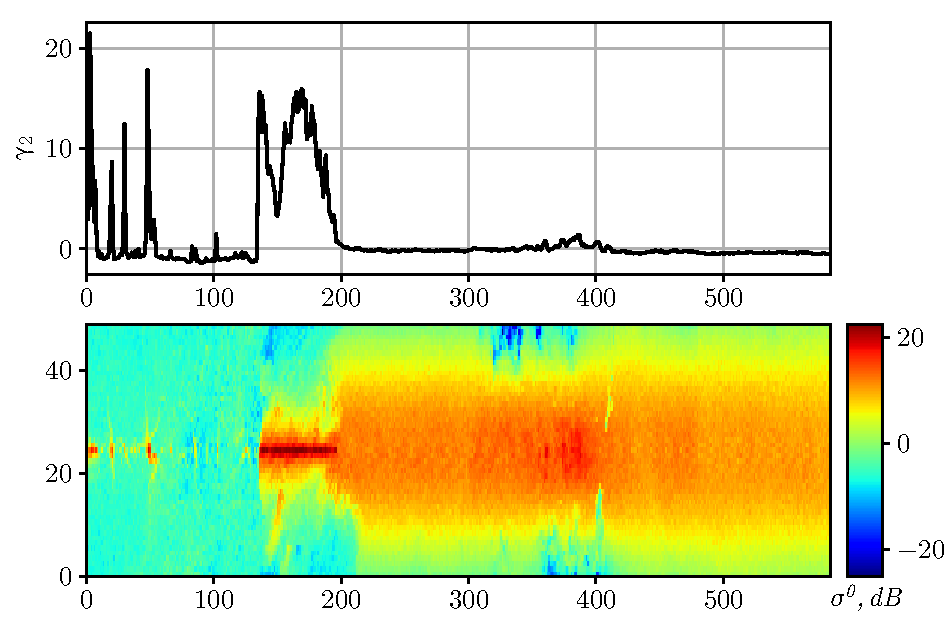
\includegraphics[width = \linewidth]{kurt.pdf}
  \caption{Сверху - коэффициент эксцесса $\gamma_2$ в зависимости от продольного номера разреза, снизу - трек данных}
  \label{fig:6}
\end{figure}

Как видно из рис. \ref{fig:6}, коэффициент эксцесса для воды (область справа от номера 200) практически равен нулю, как
и должно быть для нормального распределения. В области номеров [0,~130], географически находится
земля, ее можно убрать из рассмотрения и не обрабатывать. В области номеров [~130,~200] находится ледяной покров, и на  рис. \ref{fig:6}
видно, что для этой области коэффициент эксцесса значительно больше нуля, что позволяет численно отличить ледяную поверхность.

Однако рассчет коэффициента эксцесса дает очень грубое приближение о местонахождении льда. При таком рассчете,
используется вся ширина поперечного разреза, которая аналогична 245 км на поверхности Земли, и маркировка идет по
таким полосам. Визуально это представлено ни рис. \ref{fig:7}, где изначальный трек данных сохраняет ширину, но цветом
характеризуется не значение $\sigma^0$, а коэффициент эксцесса $\gamma_2$.

\begin{figure}[h!]
  \centering
  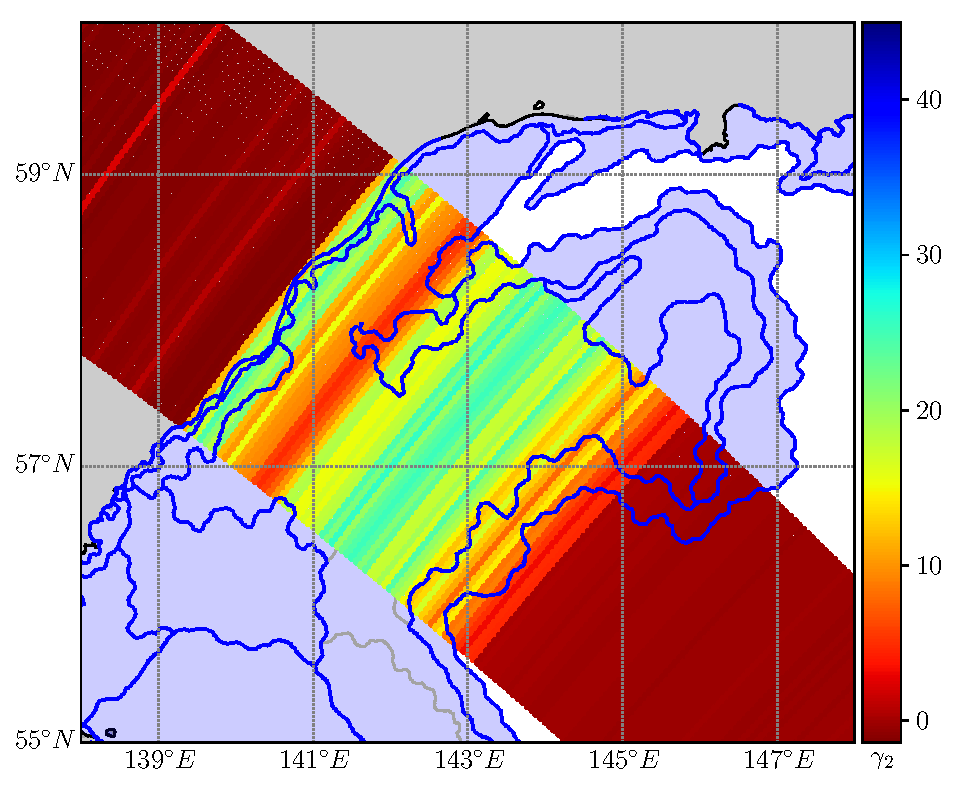
\includegraphics[width = .5\linewidth]{kurt2.pdf}
  \caption{Something}
  \label{fig:7}
\end{figure}

\textcolor{red}{Дальше курсовая не обрабатывалась, там только текст выступления}
\subsection{Детектирование границ}
Один из способов уточнить наше грубое приближение, это найти границы ледяного покрова.
Для определения границ необходимо детектировать скачки сигнала. Здесь приведены зависимости УЭПР от продольной
координаты для разных углов. Для того, чтобы выявить местонахождение скачка использовался алгоритм Джона Кэнни \cite{canny} для
одномерного случая.

\begin{equation}
  S = \frac{\left|\int \limits_{-W}^{+W} G(-x) f(x) d x\right|}{n_{0} \sqrt{\int \limits_{-W}^{+W} f^{2}(x) d x}} \frac{\left|\int \limits_{-W}^{+W} G^{\prime}(-x) f^{\prime}(x) d x\right|}{\sqrt{\int \limits_{-W}^{+W} f^{\prime 2}(x) d x}}
  \label{eq:S}
\end{equation}

\begin{equation}
  f(x) = -x\cdot \exp(-\frac{x^2}{2\sigma^2_g})
  \label{eq:fx}
\end{equation}

Рассмотрим для примера нулевой угол падения. Метод заключается в произведении двух сверток сигнала и
функции-детектора $f(x)$, результат которых здесь обозначен как S. В качестве функции-детектора выступала вторая производная от
Гауссового распределения.  Локальные максимумы функции S, соответствуют скачкам сигнала, или в нашем случае, переходам
между различающимися по характеру рассеивания поверхностями. Например здесь, первый максимум отвечает за переход
земля-лед, а второй, слабее – за переход лед-вода. 

На чувствительность алгоритма влияет вид функции-детектора, или здесь, в частности, ширина гауссового распределения
сигма. Важно, чтобы функция-детектор полностью убиралась в окно свертки, и при этом была достаточно, но не слишком
чувствительна. Чем уже функция-детектор, тем на меньшие скачки она реагирует, из-за чего функция S может стать очень
шумной. В работе был выбран оптимальный вариант соотношения ширины окна свертки и ширины функции, для наилучшего
детектирования. 

Используя такой подход обнаружения границ, размечался каждый продольный скан исследуемого трека. 

Имея теперь карту границ и карту расположения льда, мы можем совместить их, для получения более точной картины.
Например, мы можем заполнить ограниченную область, в соответствии с ее содержанием. Т.е. если в ограниченной области
находится преимущественно лед, то мы можем, учитывая что никаких скачков и перепадов там не происходило, заполнить всю
область льдом, и получить более правдоподобную разметку.


\section{Заключение}
Как видно, есть совпадение в общих чертах, но не обошлось и без пробелов. В основном это пропуски могут происходить при
попадании на срез нескольких типов поверхности. Все вышеописанные методы в таком случае работают на несколько порядков
хуже, или не работают вовсе. Чтобы детектировать лед в таких ситуациях, можно попытаться использовать машинное обучение,
для классификации поверхности в зависимости от уэпр, угла падения, и, например даты.


В результате нашей работы был разработан алгоритм, позволяющий детектировать расположение ледяного покрова, используя
данные двухчастотного локатора спутника GPM для определения типа поверхности и границ.
Из очевидных недостатков, это неточная работа алгоритма при попадании на срез нескольких типов отражающей поверхности,
потому что в таком случае считать коэффициент эксцесса и производить аппроксимацию не имеет смысла. 
В перспективе имеется план использования этих данных для попытки реализации машинного обучения, однако это отдельная
тема, со своими проблемами и задачами, которые еще предстоит решить. 


\newpage
\addcontentsline{toc}{section}{Список литературы}
\begin{thebibliography}{99}
\bibitem{kar1} Караев В. Ю. Использование данных двухчастотного дождевого радиолокатора для мониторинга формирования
и разрушения ледяного покрова на озере Байкал в осенне-зимний период 2015/2016 г. / В.Ю. Караев, М.А. Панфилова, Е.М.
Мешков, Г.Н. Баландина, З.В. Андреева, А.А. Максимов // Современные проблемы дистанционного зондирования Земли из
космоса. 2018. Т. 15. № 1. С. 206–220
\bibitem{bassfuks} Басс Ф.Г., Фукс И.М. Рассеяние волн на статистически неровной поверхности. - Наука, 1972. - 200 с.
\bibitem{meln} Мельник Ю.А., С.Г. Зубкович. Радиолокационные методы исследования Земли. ?? Советское радио, 1980 - 7 с.
\bibitem{data} NASA STORM https://storm.pps.eosdis.nasa.gov/storm
\bibitem{land} Ландау Л.Д., Лифшиц Е.М. Теоретическая физика: т.5, Статистическая физика. - М.: Физматлит, 2005. - 616 с.
\bibitem{dpr} GPM:DPR https://pmm.nasa.gov/gpm/flight-project/dpr.
\bibitem{canny} John Canny, A computational approach to edge detection. 1986.
\end{thebibliography}

\end{document}